\documentclass[12pt, a4paper]{report}

\usepackage[margin=1in]{geometry}
\usepackage[utf8]{inputenc}
\usepackage[T1]{fontenc}

\usepackage{times}

\usepackage{float}

\usepackage{url}
\usepackage{xurl} % Avoids URLs to overfull \hbox

\usepackage{graphicx}
\graphicspath{{img/}} % global configuration
\usepackage[colorlinks=false, pdfborder={0 0 0}]{hyperref}

\usepackage{tabularray}

% To use listings
\usepackage[table, svgnames]{xcolor}
\usepackage{listings}

\title{
  Data Compression
}
\author{
  Enrico Marchionni\\
  \texttt{enrico.marchionni@studio.unibo.it}
}
\date{\today}

% Package to keep track of the total number of pages
\usepackage{lastpage}
\usepackage{fancyhdr}

\fancypagestyle{fancy}{
  \fancyhf{}
  \fancyfoot[C]{\thepage\ of \pageref{LastPage}}
  \renewcommand{\headrulewidth}{0pt}
  \renewcommand{\footrulewidth}{0.4pt}
}

\fancypagestyle{plain}{
  \fancyhf{}
  \fancyfoot[C]{\thepage\ of \pageref{LastPage}}
  \renewcommand{\headrulewidth}{0pt}
  \renewcommand{\footrulewidth}{0.4pt}
}

\pagestyle{fancy}

\usepackage[backend=biber, style=alphabetic, sorting=ydnt]{biblatex}
\addbibresource{references.bib}

\usepackage{amsthm} % to make definitions
\newtheorem{definition}{Definition}[section] % custom environment for definitions
\newtheorem{example}{Example}

% for graphs and overlaying text
\usepackage{tikz}
\usepackage{pgfplots}
\pgfplotsset{compat=1.18}
\usepackage{amsmath} % For math symbols

% for binary trees
\usepackage{forest}

\definecolor{C_comment_green}{rgb}{87, 166, 74}
\definecolor{C_keyword_blue}{RGB}{86, 156, 214}
\definecolor{C_macro_purple}{RGB}{199, 120, 221}
\definecolor{C_function_amber}{RGB}{220, 220, 100}

\lstdefinelanguage{CStyle}{
  morekeywords={
    for, while
  },
  morekeywords=[2]{ % macros
    EOF
  },
  morekeywords=[3]{ % functions
    getc, high_range, low_range, output, input_code, find_symbol_straddling_this_range, putc
  },
  sensitive=true,
  morecomment=[l]//,
  morecomment=[s]{/*}{*/},
  morestring=[b]",
  morestring=[b]',
  commentstyle=\color{C_comment_green},
  keywordstyle=\color{C_keyword_blue}\bfseries,
  keywordstyle=[2]\color{C_macro_purple}\bfseries,
  keywordstyle=[3]\color{C_function_amber}\bfseries,
  stringstyle=\color{red},
  identifierstyle=\color{black},
  basicstyle=\ttfamily,
  literate={->}{{\textcolor{black}{->}}}2
            {>=}{{\textcolor{black}{>=}}}2
            {<=}{{\textcolor{black}{<=}}}2
            {!=}{{\textcolor{black}{!=}}}2
            {==}{{\textcolor{black}{==}}}2,
}

\lstset{
  basicstyle=\ttfamily,                 % Set font type
  keywordstyle=\color{blue}\bfseries,   % Set keyword color to blue and bold
  stringstyle=\color{red},              % Set string color to red
  commentstyle=\color{C_comment_green}, % Set comment color to gray and italic
  breaklines=true,                      % Enable line breaking
  frame=single,                         % Add a frame around the code
  numbers=left,                         % Add line numbers on the left
  numberstyle=\tiny\color{gray},        % Style for line numbers
  backgroundcolor=\color{lightgray!20}, % Background color
  captionpos=b,                         % Caption position at the bottom
  showstringspaces=false                % Don't show spaces in strings
}

\begin{document}

\maketitle

\begin{abstract}

Data compression is intended as the practice of reducing the size of binary digital data.
It could be considered as a procedure that takes a bit-stream in input and returns another bit-stream as output.
The output stream may be of equal length or shorter than the input.

The key to understand data compression is to discuss the distinction between data and information.
It can be said that data is how information is represented\footnote{ex. the number 0 can be expressed in binary as a sequence of a
certain number of zeros, from \(1\) to \(\infty\), and we know that calculators use at least 8 bits, let's say \(n\)
(considering it as a multiple of 8), to represent an integer number. So at the end \(n - 1\) bits are redundant in the 0
representation on a calculator.}. In simple terms, data can be compressed because its original representation is not the shortest
possible. The goal of data compression is to reduce data by maintaining the same information.

The counterpart is that in our time data is intrinsically redundant. And this redundancy is needed.
So data compression isn't only a procedure that goes from a bit-stream to another one not longer, but it requires also another
procedure that regenerates the original bit-stream of data, necessary for practical use, from the previously given output
bit-stream of information.

This makes clear that the task of compression consists of two components, an \textit{encoding} algorithm that takes a message
and generates a “compressed” representation (hopefully with fewer bits), and a \textit{decoding} algorithm that reconstructs
the original message or some approximation of it from the compressed representation.

\dots % difference between information and meaning???

\end{abstract}

\tableofcontents

\chapter{Information Theory}

In 1948, Shannon\footnote{Claude Elwood Shannon (1916-2001) was an American mathematician, electrical engineer, computer
scientist, cryptographer and inventor known as the "father of information theory".}, while working at the Bell Telephone
Laboratories, published "A Mathematical Theory of Communication" \cite{AMathematicalTheoryOfCommunication}, a seminal paper that
marked the birth of information theory. In that paper, Shannon defined the concept of "information" and proposed a precise way to
quantify it-in his theory, the fundamental unit of information is the bit.

Moreover, this discipline plays behind the concepts of entropy, randomness and data compression, all topics that will be discussed
later on.

\section{Quantifying Information}

For what concerns data compression, information of theory has developed a usable measure of the information we get from observing
the occurrence of an event having probability \(p\). Therefore information is defined in terms of the probability.

The information measure \(I(p)\) has to match the following axioms (from \cite{AnIntroductionToInformationTheoryAndEntropy}):

\begin{itemize}
  \item Information is non negative: \(I(p) \geq 0\).
  \item If an event has probability 1, we get no information: \(I(1) = 0\).
  \item If two independent events occur (whose probability is the product of their individual probabilities), then the information
  we get from observing the events is the sum of the two computed individually: \(I(p_1 \cdot p_2) = I(p_1) + I(p_2)\).
  \item Information measure must be continuous and monotonic (slight changes in probability should result in slight changes in
  information).
\end{itemize}

Considering the previous properties as axioms it can be said that: \(I(p^2) = I(p \cdot p) = I(p) + I(p) = 2 \cdot I(p)\).
Thus: \(I(p^n) = n \cdot I(p)\) (by induction).
Then: \(I(p) = I(p^{(\frac{1}{m})^m}) = m \cdot I(p^{\frac{1}{m}})\), so \(I(p^{\frac{1}{m}}) = \frac{1}{m} \cdot I(P)\),
therefore: \(I(p^{\frac{n}{m}}) = \frac{n}{m} \cdot I(p)\).
In general, considering \(r\) as a real number: \(I(p^a) = a \cdot I(p)\).

From this analysis it was discovered that:

\begin{equation} \label{eq:information1}
  I(p) = - \log_b p \ (= \log_b \frac{1}{p})
\end{equation}

Where: \(p = b_1^{\log_{b_1} p}\) and therefore: \(\log_{b_2} p = \log_{b_2} b_1^{\log_{b_1} p} = \log_{b_2} b_1 \cdot \log_{b_1}
p\). So: \(\log_{b_2} b_1\) is a constant, a scaling factor.
From another point of view it is a simple change in the unit of measurement.

For this reason:

\begin{equation} \label{eq:information2}
  I(p) = - \log_2 p
\end{equation}

\autoref{eq:information2} is the same expression of \autoref{eq:information1} where the unit of measurement is called bits
(look at \autoref{tab:information_units}). \autoref{eq:information1} was first introduced by Hartley\footnote{Ralph Vinton Lyon
Hartley (1888-1970) was an American electronics researcher. He invented the Hartley oscillator and the Hartley transform,
and contributed to the foundations of information theory.} in 1928 trying to measure uncertainty, without talking about
probability, and lately reviewed by Shannon.

\begin{table}[H]
  \begin{tblr}{
      colspec={*{2}{Q[l]}X[l]},
      width=\textwidth,
      row{odd}={gray!15},
      row{even}={white},
      row{1}={bg=gray!90,fg=white},
      colsep=4pt
    }
      \textbf{Unit of measurement} & \textbf{Base} & \\
      bit (or shannon) & \(2\) & \\
      \hline
      trit & \(3\) & \\
      \hline
      nat (natural unit of information) & \(e\) & \\
      \hline
      hartley (or dit) & \(10\) & \\
      \hline
  \end{tblr}
  \caption{\label{tab:information_units} Information units of measurement}
\end{table}

\begin{example}
Let's talk about flipping a fair coin n times. It gives us: \(- \log_2 \frac{1}{2}^n = \log_2 2^n = n \cdot \log_2 2 = n\) bits of
information. In fact a sequence of heads (coded as \(1\)) and tails (coded as \(0\)) could be expressed as: \(010010111\dots\),
these are the \(n\) bits of information.
\end{example}

\chapter{Entropy}

Entropy is a concept that was explained in many fields. Previously defined by Clausius\footnote{Rudolf Julius Emanuel Clausius
(1822-1888) was a German physicist and mathematician and is considered one of the central founding fathers of the science of
thermodynamics.} and Boltzmann\footnote{Ludwig Eduard Boltzmann (1844-1906) was an Austrian physicist and philosopher. His
greatest achievements were the development of statistical mechanics and the statistical explanation of the second law of
thermodynamics.} was later used by Shannon. It is believed that these three definitions are indeed equivalent although no formal
proof of this is available (as discussed in \cite{EntropyAndInformationTheoryUsesAndMisuses}). Informally it is advantageous to
remember that in statistical physics entropy represents the randomness or disorder of a system.

\section{Quantifying Entropy}

Here is how Shannon introduced the measure of Information:
\begin{quote}
Suppose we have a set of possible events whose probabilities of occurrence are \(p_1, p_2, \dots, p_n\). These probabilities are
known but that is all we know concerning which event will occur. Can we find a measure of how much "choice" is involved in the
selection of the event or how uncertain we are of the outcome?
\end{quote}
If there is such a measure, say, \(H(p_1, p_2, \dots, p_n)\)\footnote{Where \(H\) refers to Hartley.}, it is reasonable to require
of it the following properties:
\begin{itemize}
  \item \(H\) should be continuous in the \(p_i\).
  \item If all the \(p_i\) are equal, \(p_i = \frac{1}{n}\) then \(H\) should be a monotonic increasing function of \(n\). With
  equally likely events there is more choice, or uncertainty, when there are more possible events.
  \item If a choice be broken down into two successive choices, the original \(H\) should be the weighted sum of the individual
  values of \(H\) (The entropy of an entire stream is simply the sum of the entropy of all individual symbols).
\end{itemize}

Then Shannon proved that the only \(H\) satisfying the three assumptions above has the form:

\begin{equation} \label{eq:entropy1}
  H = -K \sum_{i = 1}^{n} p_i \ln p_i
\end{equation}

\autoref{eq:entropy1} includes a constant \(K\), in the Shannon article it is any constant. In application to thermodynamics \(K\)
turns into Boltzmann Constant. It is simply a scaling factor. Note that if \(K\) is \(\frac{1}{\ln b}\) or equivalently
\(\log_b e\), the formula, considering only \(K\) and the logarithm, becomes \(\log_b e \cdot \ln p\) that is the same of
\(\log_b e^{\ln p}\) that can be simply written as \(\log_b p\). So:

\begin{equation} \label{eq:entropy2}
  H(P) = - \sum_{i = 1}^{n} p_i \log_2 p_i
\end{equation}

Where \(P = {p_1, p_2, \dots, p_n}\) is the distribution of probability considered.
remind that in \autoref{eq:entropy2} base \(2\) could be a general base \(b\) and it can be simply view as a simple change in the
unit of measurement (as it was seen in \autoref{tab:information_units}).

An intuitive way to explain the origin of this formula is now discussed. We want to obtain the average amount of information from
each symbol we see in a stream. Let's suppose we start from \(n\) symbols \(a_1, a_1, \dots, a_n\).
A stream of these symbols is provided with probabilities \(p_1, p_1, \dots, p_n\) respectively.
As it was seen in \autoref{eq:information2} for a symbol \(a_i\) we get \(-\log_2 p_i\) information.
In a long run, say \(N\) observations, we will see (approximately) \(N \cdot p_i\) occurrences of the symbol \(a_i\).
Thus in the \(N\) independent observations, we will get total information of:

\begin{equation} \label{eq:information_entropy1}
  I = - \sum_{i = 1}^n (N \cdot p_i) \log_2 p_i
\end{equation}

So then, from \autoref{eq:information_entropy1} the average information is:

\begin{equation} \label{eq:information_entropy2}
  \frac{I}{N} = - \frac{1}{N} \sum_{i = 1}^n (N \cdot p_i) \log_2 p_i = - \sum_{i = 1}^n p_i \log_2 p_i
\end{equation}

This makes clear that entropy is a probability weighted average of the self information of each message.
At this point we get \autoref{eq:information_entropy2} that is the same as \autoref{eq:entropy2}.
Furthermore, it is shown in \autoref{eq:entropy_bounds} that \(H(P)\) is bounded (for further information see
\cite{AnIntroductionToInformationTheoryAndEntropy}):

\begin{equation} \label{eq:entropy_bounds}
  0 \leq H(P) \leq \log_2 n
\end{equation}

Larger entropies represent larger average information, and perhaps counter-intuitively, the more random a set of messages
(the more even the probabilities) the more information they contain on average.

\begin{example}

Returning to the example of the coin:

\begin{figure}[H]
  \centering
    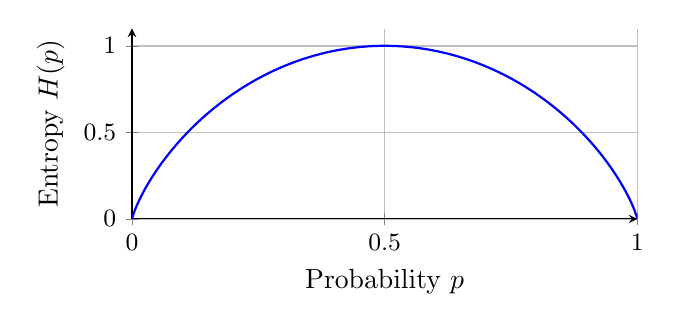
\begin{tikzpicture}
      \begin{axis}[
          width=8cm,
          height=4cm,
          xlabel={Probability \( p \)},
          ylabel={Entropy \( H(p) \)},
          ymin=0, ymax=1.1,
          xmin=0, xmax=1,
          ytick={0, 0.5, 1},
          xtick={0, 0.5, 1},
          domain=0:1,
          samples=200,
          grid=both,
          major grid style={line width=0.6pt, draw=gray!50},
          minor grid style={line width=0.3pt, draw=gray!30},
          tick label style={font=\small},
          axis lines=left
      ]
        \addplot[
          thick,
          blue,
        ]
        {-x*log2(x) - (1-x)*log2(1-x)} node[pos=0.5, above, sloped, xshift=-0.5cm, yshift=0.3cm] {};
      \end{axis}
    \end{tikzpicture}
    \caption{\label{fig:entropy_graph} Graph of entropy \( H(p) = -p \log_2(p) - (1-p) \log_2(1-p) \) for a fair coin toss.}
\end{figure}

\autoref{fig:entropy_graph} shows an example of the entropy in function of the probability of heads or tails when flipping a fair
coin.

\end{example}

\chapter{Randomness}

Compression, logically, can be interpreted as the removal of redundancy. The compressed data therefore has no structure and cannot
be distinguished from random data; in fact, it is random (\cite{AConciseIntroductionToDataCompression}).

\section{Kolmogorov}

\begin{definition}
\textbf{Kolmogorov complexity} of a binary sequence is the length of the shortest binary program that generates that sequence on a
universal Turing machine (\cite{ThreeApproachesToTheQuantitativeDefinitionOfInformation}).
\end{definition}

The concept essentially asserts that a binary sequence is considered random if there is no algorithm shorter than the sequence
itself that can generate it.

That is related to the concept of incompressibility in algorithmic randomness: a random sequence cannot be compressed into a
shorter representation than its original size.

So, loosely speaking, the randomness (or Kolmogorov complexity) of a finite sequence is equal to its shortest description.

It is known that the Kolmogorov complexity is not computable.

\section{Martin-Lof}

Martin-Lof in Algorithmic Randomness and Complexity (\cite{TheDefinitionOfRandomSequences}) shows that the random elements as
defined by Kolmogorov possess all conceivable statistical properties of randomness.

He also extended the definition for random elements with three approaches to the definition of algorithmic randomness for infinite
sequences:

\begin{definition}
The \textbf{computational paradigm}: Random sequences are those whose initial segments are all hard  to describe, or,
equivalently, hard to compress.
\end{definition}

\begin{definition}
The \textbf{measure-theoretic paradigm}: Random sequences  are those with no "effectively rare" properties. If the class of
sequences satisfying a given property is an effectively null set, then a random sequence should not have this property.
This approach is the same as the stochastic paradigm: a random sequence should pass all effective statistical tests.
\end{definition}

\begin{definition}
The \textbf{unpredictability paradigm}: This approach stems from what is probably the most intuitive conception of randomness,
namely that one should not be able to predict the next bit of a random sequence, even if one knows all preceding bits, in the same
way that a coin toss is unpredictable even given the results of previous coin tosses.
\end{definition}

Taken from \cite{AlgorithmicRandomnessAndComplexity}.

The previous citations aim to observe that the idea of Kolmogorov that random generators didn't exist was lately reviewed and
while remaining true, extended to infinite sequences.

\section{Random Sequences}

A random sequence should satisfy three conditions:

\begin{itemize}
  \item The sequence follows a uniform distribution.
  \item Each element of the sequence is independent of each other.
  \item The rest of the sequence can not be predicted from any sequence.
\end{itemize}

Random numbers can be divided into two categories: true random numbers and pseudo-random numbers.
True random number generators (RNGs) are composed of two parts: entropy source and algorithm post-processing.
Pseudo random number generators (PRNGs) take a seed as input and generate an output sequence by function.

\chapter{Data Compression}

When discussing compression algorithms it is important to make a distinction between two components: the \textbf{model} and the
\textbf{coder}.
The model component somehow captures the probability distribution of the symbols (or messages) by knowing or discovering something
about the structure of the input.
The coder component then takes advantage of the probability knowledge acquired in the model to generate codes to represent the
symbols (or messages).
It does this by effectively lengthening low probability messages and shortening high-probability messages.
It should be pointed out that the line between model and coder components of algorithms is not always well define, on the other
hand modeling and coding are two distinctly different things.

\section{Techniques}

The compression techniques can be: \textit{lossless} and \textit{lossy}.
The first category is the most similar to the theory and the most practical intuition of it.
Lossless compression ratios are generally in the range of 2:1 to 8:1.
Lossy compression, in contrast, works on the assumption that the data doesn't have to be stored perfectly.
Most information can be simply thrown away; the data will still be of acceptable quality.
This technique is frequently used in image and video compression, where a group of pixels can be approximated into a single value.
In this case the ratio can be of orders greater.
In conclusion lossless compression has a lower ratio it preserves all information that can be reload back to the original data, on
the other hand, lossy compression has a bigger ratio but it discards some information and doesn't generate the same data when it
is reloaded.

\subsection{Modeling}

It can be statistical or dictionary-based.
Statistical modeling reads in and encodes a single symbol at a time using the probability of that character's appearance.
Dictionary-based modeling uses a single code to replace strings of symbols.
This techniques can be static or adaptive.
In the second case the problem of knowing the generated structure, the table of probabilities or the dictionary,
both when encoding and when decoding, is avoided.

\subsubsection{Statistical Modeling}

It uses a static table of probabilities.
At the beginning the model was created only one time and reused for different data.
The next enhancement was to build a statistics table for every unique input stream.
The number of symbols (usually characters) is called order of the model.
In particular order-N indicates that are considered N characters before the current one.
The order is important because it determines the size of the table. The higher the order, the larger the table.
However, as the order increases, the algorithm's efficiency ratio also improves (up to the point where the overhead of
reading these tables becomes significant).
An alternative approach is to use adaptive models, that generates statistics while reading data.

\subsubsection{Dictionary Modeling}

It follows a different approach. It reads in input data and looks for groups of symbols that appear in a dictionary.
It uses pointers to refer to groups of symbols at some point in the dictionary.
The longer the match, the better the compression ratio.
In this case the modeling is the core of the compression algorithm.
Also in this case the dictionary can be static or adaptive.

\subsection{Coding}

It generate codes to represent symbols or groups of symbols.

\subsection{Implementations}

For details on these implementations and their examples, see \cite{TheDataCompressionBook2ndEdition}.

\subsubsection{Shannon-Fano coding (1950)}

Shannon at Bell Labs and Fano\footnote{Roberto Mario "Robert" Fano (1917-2016) was an Italian-American computer scientist and
professor of electrical engineering and computer science at the Massachusetts Institute of Technology.} at MIT developed this
method nearly simultaneously\footnote{This method was proposed in Shannon's "A Mathematical Theory of Communication" (1948) and
in a later technical report by Fano (1949).}.
It is necessary to know the probability of each symbol's appearance in a message.
A table of codes could be constructed that has several important properties:

\begin{itemize}
    \item Different codes have different numbers of bits.
    \item Codes for symbols with low probabilities have more bits, and codes for symbols with high probabilities have fewer bits.
    \item Though the codes are of different bit lengths, they can be uniquely decoded.
\end{itemize}

Arranging the codes as a binary tree solves the problem of decoding these variable-length codes.

The actual algorithm is:

\begin{enumerate}
    \item For a given list of symbols, develop a corresponding list of probabilities or frequency counts so that each symbol's
    relative frequency of occurrence is known.
    \item Sort the lists of symbols according to frequency, with the most frequently occurring symbols at the top and the least
    common at the bottom.
    \item Divide the list into two parts, with the total frequency counts of the upper half being as close to the total of the
    bottom half as possible.
    \item The upper half of the list is assigned the binary digit 0, and the lower half is assigned the digit 1. This means
    that the codes for the symbols in the first half will all start with 0, and the codes in the second half will all start
    with 1.
    \item Recursively apply the steps 3 and 4 to each of the two halves, subdividing groups and adding bits to the codes
    until each symbol has become a corresponding code leaf on the tree.
\end{enumerate}

\begin{example}
In the following tables the execution steps of the algorithm are explained in a specific example
(taken from \cite{TheDataCompressionBook2ndEdition}).

The input data are:

\begin{table}[H]
  \begin{tblr}{
      colspec={*{2}{Q[l]}X[l]},
      row{odd}={gray!15},
      row{even}={white},
      row{1}={bg=gray!90,fg=white},
      colsep=4pt
    }
      \textbf{Symbol} & \textbf{Count} & \\
      \textbf{A} & 15 & \\
      \hline
      \textbf{B} & 7 & \\
      \hline
      \textbf{C} & 6 & \\
      \hline
      \textbf{D} & 6 & \\
      \hline
      \textbf{E} & 5 & \\
      \hline
  \end{tblr}
  \caption{\label{tab:ex_shannon-fano_input} Input data.}
\end{table}

\autoref{tab:ex_shannon-fano_input} shows data of a widespread example about minimum redundancy
coding\footnote{It is a code constructed in such a way that the average number of coding digits per message is minimized.}.

The result of the first step is:

\begin{table}[H]
  \begin{tblr}{
      colspec={*{3}{Q[l]}X[l]},
      width=\textwidth,
      row{odd}={gray!15},
      row{even}={white},
      row{1}={bg=gray!90,fg=white},
      colsep=4pt
    }
      \textbf{Symbol} & \textbf{Count} & & \\
      \textbf{A} & 15 & \textcolor{red}{0} & \\
      \textbf{B} & 7 & \textcolor{red}{0} & \\
      \cline[1.5pt,red]{1-3}
      % \cline{4-4}
      \textbf{C} & 6 & \textcolor{red}{1} & \\
      \textbf{D} & 6 & \textcolor{red}{1} & \\
      \textbf{E} & 5 & \textcolor{red}{1} & \\
      \hline
  \end{tblr}
  \caption{\label{tab:ex_shannon-fano_output1} Shannon-Fano output of the first step.}
\end{table}

\autoref{tab:ex_shannon-fano_output1} shows with a red line the split of the first step.

The result of the other steps is:

\setlength{\arrayrulewidth}{1.5pt}
\arrayrulecolor{red}

\begin{table}[H]
  \begin{tblr}{
      colspec={*{5}{Q[l]}X[l]},
      width=\textwidth,
      row{odd}={gray!15},
      row{even}={white},
      row{1}={bg=gray!90,fg=white},
      colsep=4pt
    }
      \textbf{Symbol} & \textbf{Count} & & \\
      \textbf{A} & 15 & \textcolor{red}{0} & \textcolor{red}{0} & \\
      \cline[1.5pt,red]{1-4}
      % \cline{5-6}
      \textbf{B} & 7  & \textcolor{red}{0} & \textcolor{red}{1} & \\
      \cline[1.5pt,red]{1-3}
      % \cline{4-6}
      \textbf{C} & 6  & \textcolor{red}{1} & \textcolor{red}{0} & \\
      \cline[1.5pt,red]{1-4}
      % \cline{5-6}
      \textbf{D} & 6  & \textcolor{red}{1} & \textcolor{red}{1} & \textcolor{red}{0} & \\
      \cline[1.5pt,red]{1-5}
      % \cline{6-6}
      \textbf{E} & 5  & \textcolor{red}{1} & \textcolor{red}{1} & \textcolor{red}{1} & \\
      \hline
  \end{tblr}
  \caption{\label{tab:ex_shannon-fano_output} Shannon-Fano final output.}
\end{table}

\autoref{tab:ex_shannon-fano_output} shows with horizontal red lines the Shannon-Fano steps by showing the splits.

Another view of the structure is:

\begin{figure}[H]
  \centering
    \begin{forest}
      for tree={
        draw, % Draw a box around each node
        circle, % Node shape (can be changed to rectangle, etc.)
        minimum size=1.5em, % Size of the node
        inner sep=2pt, % Space between text and node border
        l=1.5cm, % Level distance
        s sep+=1cm, % Sibling distance
        align=center % Enable multiline text in nodes
      }
      [
        [, edge label={node[midway,left]{0}}
          [\textbf{A}, edge label={node[midway,left]{0}}]
          [\textbf{B}, edge label={node[midway,right]{1}}]
        ]
        [24, edge label={node[midway,right]{1}}
          [\textbf{C}, edge label={node[midway,left]{0}}]
          [, edge label={node[midway,right]{1}}
            [\textbf{D}, edge label={node[midway,left]{0}}]
            [\textbf{E}, edge label={node[midway,right]{1}}]
          ]
        ]
      ]
    \end{forest}
    \caption{\label{fig:ex_shannon-fano_tree} Shannon-Fano tree.}
\end{figure}

\autoref{fig:ex_shannon-fano_tree} shows the Shannon-Fano binary tree.

The symbols with higher probability of occurrence (higher count) have fewer bits in their code.

The given results can be compared with some computations about the information theory.
In the following table .

\begin{table}[H]
  \begin{tblr}{
      colspec={*{6}{X[l]}},
      width=\textwidth,
      row{odd}={gray!15},
      row{even}={white},
      row{1}={bg=gray!90,fg=white},
      colsep=4pt
    }
      \textbf{Symbol} & \textbf{Count} & \textbf{Information} & \textbf{\hyperref[eq:information2]{Number of Bits}}
       & \textbf{SF Size} & \textbf{SF Bits} \\
      \textbf{A} & 15 & \hyperref[eq:information2]{1.38} & 20.68 & 2 & 30 \\
      \hline
      \textbf{B} & 7 & \hyperref[eq:information2]{2.48} & 17.35 & 2 & 14 \\
      \hline
      \textbf{C} & 6 & \hyperref[eq:information2]{2.70} & 16.20 & 2 & 12 \\
      \hline
      \textbf{D} & 6 & \hyperref[eq:information2]{2.70} & 16.20 & 3 & 18 \\
      \hline
      \textbf{E} & 5 & \hyperref[eq:information2]{2.96} & 14.82 & 3 & 15 \\
      \hline
  \end{tblr}
  \caption{\label{tab:ex_shannon-fano_information} Information for each symbol.}
\end{table}

\autoref{tab:ex_shannon-fano_information} shows the amount of \textbf{Information} that is computed with
\autoref{eq:information2}, while the \textbf{Number of Bits} is computed with \(count \cdot \autoref{eq:information2}\)

\end{example}

\subsubsection{Huffman coding (1952)}

It is similar to the Shannon-Fano coding. It was introduced two years later then the Shannon-Fano coding.
It was first published his 1952 paper, "A Method for the Construction of Minimum Redundancy Codes".
It is more efficient than the other one.
The Shannon-Fano tree is built top-down, starting by assigning the most significant bits to each code and working down
the tree until finished.
Instead, Huffman codes are constructed bottom-up, beginning with the tree's leaves and progressing toward its root.

The tree is then built with the following steps:

\begin{itemize}
    \item The two free nodes with the lowest weights are located.
    \item A parent node for these two nodes is created. It is assigned a weight equal to the sum of the two child nodes.
    \item The parent node is added to the list of free nodes, and the two child nodes are removed from the list.
    \item One of the child nodes is designated as the path taken from the parent node when decoding a 0 bit.
    The other is arbitrarily set to the 1 bit.
    \item The previous steps are repeated until only one free node is left. This free node is designated the root of the tree.
\end{itemize}

\begin{example}

Reconsidering the \autoref{tab:ex_shannon-fano_input} input let's apply the Huffman coding algorithm.
The result is shown:

\begin{figure}[H]
  \centering
    \begin{forest}
      for tree={
        draw,
        circle,
        minimum size=1.5em,
        inner sep=2pt,
        l=1.5cm,
        s sep+=1cm,
        align=center
      }
      [39
        [{\textbf{A}\\15}, edge label={node[midway,left]{0}}]
        [24, edge label={node[midway,right]{1}}
          [13, edge label={node[midway,left]{0}}
            [{\textbf{B}\\7}, edge label={node[midway,left]{0}}]
            [{\textbf{C}\\6}, edge label={node[midway,right]{1}}]
          ]
          [11, edge label={node[midway,right]{1}}
            [{\textbf{D}\\6}, edge label={node[midway,left]{0}}]
            [{\textbf{E}\\5}, edge label={node[midway,right]{1}}]
          ]
        ]
      ]
    \end{forest}
    \caption{\label{fig:ex_huffman_tree} Huffman tree.}
\end{figure}

\autoref{fig:ex_huffman_tree} shows the Huffman binary tree, this can be compared with \autoref{fig:ex_shannon-fano_tree}.

The codes generated are:

\begin{table}[H]
  \begin{tblr}{
      colspec={*{2}{X[l]}},
      width=\textwidth,
      row{odd}={gray!15},
      row{even}={white},
      row{1}={bg=gray!90,fg=white},
      colsep=4pt
    }
      \textbf{Symbol} & \textbf{Code} & \\
      \textbf{A} & 0 \\
      \hline
      \textbf{B} & 100 \\
      \hline
      \textbf{C} & 101 \\
      \hline
      \textbf{D} & 110 \\
      \hline
      \textbf{E} & 111 \\
      \hline
  \end{tblr}
  \caption{\label{tab:ex_huffman_codes} The Huffman codes table.}
\end{table}

\autoref{tab:ex_huffman_codes} shows them.

A comparison between this example for Shannon-Fano and Huffman codes follows:

\begin{table}[H]
  \begin{tblr}{
      colspec={*{6}{X[l]}},
      width=\textwidth,
      row{odd}={gray!15},
      row{even}={white},
      row{1}={bg=gray!90,fg=white},
      colsep=4pt
    }
      \textbf{Symbol} & \textbf{Count} & \textbf{Shannon-Fano Code Length} & \textbf{Shannon-Fano Bits}
       & \textbf{Huffman Code Length} & \textbf{Huffman Bits} \\
      \textbf{A} & 15 & 2 & 30 & 1 & 15 \\
      \hline
      \textbf{B} & 7 & 2 & 14 & 3 & 21 \\
      \hline
      \textbf{C} & 6 & 2 & 12 & 3 & 18 \\
      \hline
      \textbf{D} & 6 & 3 & 18 & 3 & 18 \\
      \hline
      \textbf{E} & 5 & 3 & 15 & 3 & 15 \\
      \hline
  \end{tblr}
  \caption{\label{tab:ex_shannon-fano_huffman_comparision} Information for each symbol.}
\end{table}

\autoref{tab:ex_shannon-fano_huffman_comparision} shows that Huffman is better than Shannon-Fano because it uses less bits.
As a matter of fact, for a message with an information content of 85.25 bits, Shannon-Fano coding requires 89 bits, but Huffman
coding requires only 87.

\end{example}

\subsubsection{Arithmetic coding (1976)}

Basic algorithms for arithmetic coding were developed independently by Jorma J. Rissanen\footnote{Jorma Johannes Rissanen
(1932-2020) was an information theorist, known for originating the minimum description length (MDL) principle and practical
approaches to arithmetic coding for lossless data compression.}, at IBM Research, and by Richard C. Pasco, a Ph.D. student at
Stanford University; both were published in May 1976.

Huffman coding is a fixed-length coding method available and it is the best available.
Nevertheless Huffman codes have to be an integral number of bits long, and this can sometimes be a problem.
If the probability of a character is 1/3, for example, the optimum number of bits to code that character is around 1.6 bits.
Huffman coding has to assign either one or two bits to the code, and either choice leads to a longer compressed message than is
theoretically possible. In fact Huffman is a non optimal coding technique.

Arithmetic coding bypasses the idea of replacing an input symbol with a specific code.
It replaces a stream of input symbols with a single floating-point output number.

\begin{example}

The message "BILL GATES", for example, would have the following probability distribution:

\begin{table}[H]
  \begin{tblr}{
      colspec={*{3}{X[l]}},
      width=\textwidth,
      row{odd}={gray!15},
      row{even}={white},
      row{1}={bg=gray!90,fg=white},
      colsep=4pt
    }
      \textbf{Symbol} & \textbf{Probability} & \textbf{Range} \\
      \textbf{` '} & 1/10 & \(0 < r < 0.1\) \\
      \hline
      \textbf{A} & 1/10 & \(0.1 < r < 0.2\) \\
      \hline
      \textbf{B} & 1/10 & \(0.2 < r < 0.3\) \\
      \hline
      \textbf{E} & 1/10 & \(0.3 < r < 0.4\) \\
      \hline
      \textbf{G} & 1/10 & \(0.4 < r < 0.5\) \\
      \hline
      \textbf{I} & 1/10 & \(0.5 < r < 0.6\) \\
      \hline
      \textbf{L} & 2/10 & \(0.6 < r < 0.8\) \\
      \hline
      \textbf{S} & 1/10 & \(0.8 < r < 0.9\) \\
      \hline
      \textbf{T} & 1/10 & \(0.9 < r < 1\) \\
      \hline
  \end{tblr}
  \caption{\label{tab:ex_arithmetic_input} Input data.}
\end{table}

\autoref{tab:ex_arithmetic_input} shows input data, how the are sorted and their range of probability.

The Arithmetic coding encoding algorithm is:

\begin{lstlisting}[language=CStyle, caption={Arithmetic coding encoding algorithm}, label={lst:ex_arithmetic_encoding}]
  low = 0.0;
  high = 1.0;
  while ((c = getc(input)) != EOF) {
    range = high - low;
    high = low + range * high_range(c);
    low = low + range * low_range(c);
  }
  output(low);
\end{lstlisting}

Following the encoding process shown in \autoref{lst:ex_arithmetic_encoding} brings to the following result:

\begin{table}[H]
  \begin{tblr}{
      colspec={*{3}{X[l]}},
      width=\textwidth,
      row{odd}={gray!15},
      row{even}={white},
      row{1}={bg=gray!90,fg=white},
      colsep=4pt
    }
      \textbf{Symbol} & \textbf{Low Value} & \textbf{High Value} \\
       & 0.0 & 1.0 \\
      \hline
      \textbf{B} & 0.2 & 0.3 \\
      \hline
      \textbf{I} & 0.25 & 0.26 \\
      \hline
      \textbf{L} & 0.256 & 0.258 \\
      \hline
      \textbf{L} & 0.2572 & 0.2576 \\
      \hline
      \textbf{` '} & 0.2572 & 0.25724 \\
      \hline
      \textbf{G} & 0.257216 & 0.25722 \\
      \hline
      \textbf{A} & 0.2572164 & 0.2572168 \\
      \hline
      \textbf{T} & 0.25721676 & 0.2572168 \\
      \hline
      \textbf{E} & 0.257216772 & 0.257216776 \\
      \hline
      \textbf{S} & 0.2572167752 & 0.2572167756 \\
      \hline
  \end{tblr}
  \caption{\label{tab:ex_arithmetic_encoding} Arithmetic encoding.}
\end{table}

So the final value 0.2572167752 (as shown in \autoref{tab:ex_arithmetic_encoding}), will uniquely encode "BILL GATES".

The Arithmetic coding decoding algorithm is:

\begin{lstlisting}[language=CStyle, caption={Arithmetic coding encoding algorithm}, label={lst:ex_arithmetic_decoding}]
  number = input_code();
  for (;;) {
    symbol = find_symbol_straddling_this_range(number);
    putc(symbol);
    range = high_range(symbol) - low_range(symbol);
    number = number - low_range(symbol);
    number = number / range;
  }
\end{lstlisting}

Following the decoding process shown in \autoref{lst:ex_arithmetic_decoding} brings to the following result:

\begin{table}[H]
  \begin{tblr}{
    colspec={*{5}{X[l]}},
    width=\textwidth,
    row{odd}={gray!15},
    row{even}={white},
    row{1}={bg=gray!90,fg=white},
    colsep=4pt
  }
    \textbf{Encoded Number} & \textbf{Output Symbol} & \textbf{Low Value} & \textbf{High Value} & \textbf{Range} \\
    0.2572167752 & \textbf{B} & 0.2 & 0.3 & 0.1 \\
    \hline
    0.572167752 & \textbf{I} & 0.5 & 0.6 & 0.1 \\
    \hline
    0.72167752 & \textbf{L} & 0.6 & 0.8 & 0.2 \\
    \hline
    0.6083876 & \textbf{L}  & 0.6 & 0.8 & 0.2 \\
    \hline
    0.041938 & \textbf{` '} & 0.0 & 0.1 & 0.1 \\
    \hline
    0.41938 & \textbf{G} & 0.4 & 0.5 & 0.1 \\
    \hline
    0.1938 & \textbf{A} & 0.2 & 0.3 & 0.1 \\
    \hline
    0.938 & \textbf{T} & 0.9 & 1 & 0.1 \\
    \hline
    0.38 & \textbf{E} & 0.3 & 0.4 & 0.1 \\
    \hline
    0.8 & \textbf{S} & 0.8 & 0.9 & 0.1 \\
    \hline
    0 & & & & \\
    \hline
  \end{tblr}
  \caption{\label{tab:ex_arithmetic_decoding} Arithmetic decoding.}
\end{table}

In summary, the encoding process is simply one of narrowing the range of possible numbers with every new symbol.
The new range is proportional to the predefined probability attached to that symbol.
Decoding is the inverse procedure, in which the range is expanded in proportion to the probability of each symbol as it is
extracted (see \autoref{tab:ex_arithmetic_decoding}).

\end{example}

\paragraph{Practical Matters}

Encoding and decoding a stream of symbols using arithmetic coding at first glance seems completely impractical.
Particularly because floating point numbers have many limitations on digital computers.
As it turns out, arithmetic coding is best accomplished using integer math.
Floating point math is not required.

\subsubsection{LZ77 (1977)}

Ziv and Lempel paper: "A Universal Algorithm for Sequential Data Compression" was published in 1977 inside IEEE Transactions on
Information Theory.
LZ77 is revolutionary because that compression uses previously seen text as a dictionary.
It achieves compression by replacing variable-length strings in the input text with fixed-size pointers into the dictionary.

The main data structure in LZ77 is a text window, divided into two parts.
The first consists of a large block of recently decoded text.
The second, normally much smaller, is a look-ahead buffer.
The look-ahead buffer has characters read in from the input stream but not yet encoded.

The normal size of the text window is several thousand characters.
The look-ahead buffer is generally much smaller, maybe ten to one hundred characters.
The algorithm tries to match the contents of the look-ahead buffer to a string in the dictionary.

LZ77 encodes in sequences of tokens.
Each token consists of three items:

\begin{enumerate}
  \item An offset to a phrase in the text window.
  \item The length of the phrase.
  \item The first symbol in the look-ahead buffer that follows the phrase.
\end{enumerate}

The decompression algorithm is very similar to the previous one.
It reads in a token, outputs the indicated phrase, outputs the following character, shifts, and repeats.
It maintains the window, but it does not work with string comparisons.

\subsubsection{LZ78 (1978)}

Ziv and Lempel paper: "Compression of Individual Sequences via Variable-Rate Coding" was published in 1978 inside IEEE
Transactions on Information Theory.

LZ78 abandons the concept of a text window.
Under LZ78, the dictionary is a potentially unlimited list of previously seen phrases.
LZ78 also outputs a series of tokens with essentially the same meanings of LZ77.
Unlike LZ77, the phrase length is not passed since the decoder knows it.

LZ78 adds that phrase to the dictionary.
After the phrase is added, it will be available to the encoder at any time in the future, not just for the next few thousand
characters.

This algorithm is "greedy", so it takes locally optimal decision optimal choice at each stage.
The problem is that in many cases, like in this one, a greedy strategy does not produce an optimal solution.

\begin{example}

Consider the following input text: "DAD DADA DADDY DADO...".

\begin{table}[H]
  \begin{tblr}{
      colspec={*{3}{Q[l]}X[l]},
      width=\textwidth,
      row{odd}={gray!15},
      row{even}={white},
      row{1}={bg=gray!90,fg=white},
      colsep=4pt
    }
      \textbf{Output Phrase} & \textbf{Output Character} & \textbf{Encoded String} & \\
      0 & D & D & \\
      \hline
      0 & A & A & \\
      \hline
      1 & ` ' & `D ' & \\
      \hline
      1 & A & DA & \\
      \hline
      4 & ` ' & `DA ' & \\
      \hline
      4 & D & DAD & \\
      \hline
      1 & Y & DY & \\
      \hline
      0 & ` ' & ` ' & \\
      \hline
      6 & O & DADO & \\
      \hline
  \end{tblr}
  \caption{\label{tab:ex_arithmetic_encoding} Arithmetic encoding.}
\end{table}

Each new phrase that was not seen before is also added to the dictionary that initially was empty.
Step by step the dictionary helps to reduce the volume of data.

\end{example}

The previous example makes clear that the decompression is done without giving the dictionary to the decompressor, because the
compression algorithm always outputs the phrase and character components of a code before it uses them.
This is very important because in this way the compressed data is not burdened with carrying a large dictionary.

\section{Comparison of Algorithms}

They are useful when done on algorithms of the same compression technique: lossless or lossy.
The following factors refer mainly to lossless data compression, in the lossy case it is more complicated (for example it should
be considered how good is the approximation).
Measurements have to be considered as averages in practice, because they are different for every single sample so their value is
an approximation.

\subsection{Compression Ratio}

An important factor when considering data compression is the "compression ratio". It is simply the sample size reduction factor
(look at \autoref{eq:factor_compression_ratio}).

\begin{equation} \label{eq:factor_compression_ratio}
  compression ratio = \frac{uncompressed file size}{compressed file size}
\end{equation}

\subsection{Compression Speed}

It is important is specific use cases, usually when the network is involved (look at \autoref{eq:factor_decompression_speed}).

\begin{equation} \label{eq:factor_compression_speed}
  compression speed (MB / s) = \frac{uncompressed file size (MB)}{compression time (s)}
\end{equation}

\subsection{Decompression Speed}

As the compression speed, it is important is specific use cases, usually when the network is involved (look at
\autoref{eq:factor_decompression_speed}).

\begin{equation} \label{eq:factor_decompression_speed}
  decompression speed (MB / s) = \frac{uncompressed file size (MB)}{uncompression time (s)}
\end{equation}

\chapter{Compression Tools}

\dots

\appendix

\printbibliography

\end{document}
